\documentclass{article}
\usepackage[a4paper, margin=.5in]{geometry}
\usepackage{amssymb}
\usepackage{graphicx}
\graphicspath{ {./images/} }

\title{Submission 3.2}
\date{}
\begin{document}
\maketitle
\begin{enumerate}
      \item Let $f:A \to B$. Let $A_{0} \subset A$ and $B_{0} \subset B$.
            \begin{enumerate}
                  \item Show that $A_{0} \subset f^{-1}(f(A_{0}))$ and that equality holds if $f$ is injective.\\

                        Proof that $A_{0} \subset f^{-1}(f(A_{0}))$:\\
                        By the definition of an inverse, $f^{-1}(C) = \{x \mid f(x) \in C\}$. Thus, $f^{-1}(f(A_{0})) = \{x \mid f(x) \in f(A_{0})\}$.\\
                        For every $a \in A_{0}$, $f(a) \in f(A_{0})$, fulfilling the conditions of the set.\\
                        Therefore, $A_{0} \subset f^{-1}(f(A_{0}))$.\\

                        Proof that $A_{0} = f^{-1}(f(A_{0}))$ if $f$ is injective:\\
                        By the definition of an inverse, $f^{-1}(f(A_{0})) = \{x \mid f(x) \in f(A_{0})\}$.\\
                        Let $a \in f^{-1}(f(A_{0}))$. Therefore, $f(a) \in f(A_{0})$. Therefore, there is some $x \in A_{0}$ such that $f(a) = f(x)$.\\
                        By the definition of injectivity, $f(a) = f(x)$ implies that $a = x$.\\
                        Therefore, for every $a \in f^{-1}(f(A_{0}))$, $a = x \in A_{0}$. Thus, $f^{-1}(f(A_{0})) \subset A_{0}$. As proven above, $A_{0} \subset f^{-1}(f(A_{0}))$ as well, so $A_{0} = f^{-1}(f(A_{0}))$.

                  \item Show that $f(f^{-1}(B_{0})) \subset B_{0}$ and that equality holds if $f$ is surjective.\\

                        Proof that $f(f^{-1}(B_{0})) \subset B_{0}$:\\
                        By the definition of a function, $f(f^{-1}(B_{0})) = \{x \mid f^{-1}(x) \in f^{-1}(B_{0})\}$ and by the definition of an inverse, $f^{-1}(B_{0}) = \{x \mid f(x) \in B_{0}\}$.\\
                        For every element $b \in f(f^{-1}(B_{0})), f^{-1}(b) \in f^{-1}(B_{0})$. Therefore (by assigning $x = f^{-1}(b)$), $f(f^{-1}(b)) \in B_{0}$.\\
                        This means $f(f^{-1}(B_{0})) \subset B_{0}$.\\

                        An alternate (and probably better) proof:\\
                        By the definition of an inverse, $f^{-1}(B_{0}) = \{x \mid f(x) \in B_{0}\}$.\\
                        Let $x \in f^{-1}(B_{0})$. By definition, $f(x) \in B_{0}$, so $f^{-1}(B_{0}) \subset B_{0}$.\\

                        Proof that $f(f^{-1}(B_{0})) = B_{0}$ if $f$ is surjective:\\
                        % By the definition of an inverse, $f(f^{-1}(B_{0})) = \{x \mid f^{-1}(x) \in f^{-1}(B_{0})\}$ and $f^{-1}(B_{0}) = \{x \mid f(x) \in B_{0}\}$.\\
                        % % For every $b \in f(f^{-1}(B_{0}))$, there exists some $x \in B_{0}$ such that $f^{-1}(b) = f^{-1}(x)$.\\
                        % $B_{0} \subset B$, so $b \in B_{0} \Rightarrow b \in B$. By the definition of surjectivity, this means that for every $b$ in $B_{0}$, there is some $a \in A_{0}$ such that $b = f(a)$.\\
                        % Every $f(a) \in f(A_{0})$, so every $b \in B_{0}$ is also an element of $f(A_{0})$, so $B_{0} \subset f(A_{0})$.\\
                        % \*Insert a proof that $A_{0} \subset f^{-1}(B_{0})$* IDK, I'm losing braincells.\\\\
                        % Attempt 2:\\
                        Let $b \in B_{0}$. By the definition of surjectivity, there exists an $x$ such that $b = f(x)$. By the definition of an inverse, $f^{-1}(b) = x$. Therefore, $b = f(x) = f(f^{-1}(b))$. Thus, every element $b \in B_{0}$ is equal to an element $f(f^{-1}(b)) \in f(f^{-1}(B_{0}))$, so $B_{0} \subset f(f^{-1}(B_{0}))$. As proven above, $f(f^{-1}(B_{0})) \subset B_{0}$, so $f(f^{-1}(B_{0})) = B_{0}$.

            \end{enumerate}
      \item Let $f:A \to B$ and let $A_{i} \subset A$ and $B_{i} \subset B$ for $i = 0$ and $i = 1$. Show that $f^{-1}$ preserves inclusions, unions, intersections, and differences of sets.
            \begin{enumerate}
                  \item $B_{0} \subset B_{1} \Rightarrow f^{-1}(B_{0}) \subset f^{-1}(B_{1})$\\
                        Let $x \in f^{-1}(B_{0})$. By the definition of an inverse, $f(x) \in B_{0}$. Because $B_{0} \subset B_{1}$, $f(x) \in B_{1}$ as well.\\
                        $f^{-1}(B_{1}) = \{x \mid f(x) \in B_{1}\}$. Thus, every element in $f^{-1}(B_{0})$ is also in $f^{-1}(B_{1})$, so $f^{-1}(B_{0}) \subset f^{-1}(B_{1})$.
                  \item $f^{-1}(B_{0} \cup B_{1}) = f^{-1}(B_{0})\cup f^{-1}(B_{1})$\\
                        Let $x \in f^{-1}(B_{0} \cup B_{1})$. By the definition of an inverse, $f(x) \in B_{0} \cup B_{1}$, so $f(x) \in B_{0} \lor f(x) \in B_{1}$.\\
                        Let $y \in f^{-1}(B_{0})\cup f^{-1}(B_{1})$. By the deinition of inverses, this means $f(y) \in B_{0} \lor f(y) \in B_{1}$.\\
                        Since the definitions for being contained in either set are the same, the two sets are equivalent.
                  \item $f^{-1}(B_{0} \cap B_{1}) = f^{-1}(B_{0})\cap f^{-1}(B_{1})$\\
                        Let $x \in f^{-1}(B_{0} \cap B_{1})$. $f(x) \in B_{0} \cap B_{1}$, so $f(x) \in B_{0} \land f(x) \in B_{1}$. This can be rewritten as $f^{-1}(B_{0})\cap f^{-1}(B_{1})$ and all steps are reversible, showing equality.
                  \item $f^{-1}(B_{0} - B_{1}) = f^{-1}(B_{0}) - f^{-1}(B_{1})$\\
                        Let $x \in f^{-1}(B_{0} - B_{1})$. $f(x) \in B_{0} - B_{1}$, so $x \in B_{0} \land x \notin B_{1}$. This can be rewritten as $f^{-1}(B_{0}) - f^{-1}(B_{1})$ and all steps are reversible, again showing equality.
            \end{enumerate}
            Show that $f$ preserves inclusions and unions only:
            \begin{enumerate}
                  \setcounter{enumii}{4}
                  \item $A_{0} \subset A_{1} \Rightarrow f(A_{0})  \subset f(A_{1})$\\
                        % Let $x \in A_{0}$. $f(x) \in f(A_{0})$. However, because $A_{0} \subset A_{1}$, $x \in A_{1}$, so $f(x) \in f(A_{1})$ as well. Every $f(x) \in f(A_{0})$ corresponds to at least one $x \in A_{0}$, so $f(A_{0})  \subset f(A_{1})$.\\
                        Let $b \in f(A_{0})$. There is some $x \in A_{0}$ such that $f(x) = a$. Because $A_{0} \subset A_{1}$, $x \in A_{1}$, so $f(x) \in f(A_{1})$. Thus, every $a \in f(A_{0})$ is also in $f(A_{1})$, so $f(A_{0}) \subset f(A_{1})$.
                  \item $f(A_{0} \cup A_{1}) = f(A_{0}) \cup f(A_{1})$\\
                        Let $b \in f(A_{0} \cup A_{1})$. There exists some $x \in A_{0} \cup A_{1}$ such that $f(x) = b$. $x \in A_{0} \cup A_{1}$ is logically equivalent to $x \in A_{0} \lor x \in A_{1}$. Thus, $f(x) \in f(A_{0}) \lor f(x) \in A_{1}$, so $f(x) \in f(A_{0}) \cup f(A_{1})$. Substituting $b$ back in for $f(x)$, we get $b \in f(A_{0}) \cup f(A_{1})$. Because every step is reversible, $f(A_{0} \cup A_{1}) = f(A_{0}) \cup f(A_{1})$.
                  \item $f(A_{0} \cap A_{1}) \subset f(A_{0}) \cap f(A_{1})$\\
                        Let $b \in f(A_{0} \cap A_{1})$. There exists some $x \in A_{0} \cap A_{1}$ such that $f(x) = b$. This means that $x \in A_{0} \land x \in A_{1}$, so $f(x) \in f(A_{0}) \land f(x) \in f(A_{1})$, so $f(x) \in f(A_{0}) \cap f(A_{1})$. Thus, every $b \in f(A_{0} \cap A_{1})$ is also in $f(A_{0}) \cap f(A_{1})$, so $f(A_{0} \cap A_{1}) \subset f(A_{0}) \cap f(A_{1})$.\\

                        Show that equality holds if $f$ is injective.\\
                        Let $b \in f(A_{0}) \cap f(A_{1})$. $b \in f(A_{0}) \land b \in f(A_{1})$. There exists an $x_{0} \in A_{0}$ such that $f(x_{0}) = b$ and an $x_{1} \in A_{1}$ such that $f(x_{1}) = b$. Thus, $f(x_{0}) = f(x_{1})$. By the definition of injectivity, $x_{0} = x_{1}$. Thus, $x_{0} \in A_{0} \land x_{0} \in A_{1}$, so $x_{0} \in A_{0} \cap A_{1}$, so $f(x_{0}) \in f(A_{0} \cap A_{1})$. Thus, every $b \in f(A_{0}) \cap f(A_{1})$ is also in $f(A_{0} \cap A_{1})$, so $f(A_{0}) \cap f(A_{1}) \subset f(A_{0} \cap A_{1})$. As shown above, $f(A_{0} \cap A_{1}) \subset f(A_{0}) \cap f(A_{1})$, so $f(A_{0} \cap A_{1}) = f(A_{0}) \cap f(A_{1})$.
                  \item $f(A_{0} - A_{1}) \supset f(A_{0}) - f(A_{1})$\\
                        Let $b \in f(A_{0}) - f(A_{1})$. $b \in f(A_{0}) \land b \notin f(A_{1})$. This means there exists an $x_{0} \in A_{0}$ such that $f(x_{0}) = b$, and there does not exist an $x_{1} \in A_{1}$ such that $f(x_{1}) = b$. Thus, for any $x$ such that $f(x) = b$, $x \in A_{0} \land x \notin A_{1}$, so $x \in A_{0} - A_{1}$. Therefore, every $b \in f(A_{0}) - f(A_{1})$ is also in $f(A_{0} - A_{1})$, so $f(A_{0} - A_{1}) \supset f(A_{0}) - f(A_{1})$.\\

                        Show that equality holds if $f$ is injective.\\
                        Let $b \in f(A_{0} - A_{1})$. There exists an $x \in A_{0} - A_{1}$ such that $f(x) = b$. Thus, $x \in A_{0} \land x \notin A_{1}$. Let there be some $a \in A_{1}$ such that $f(a) = b = f(x)$. However, because $f$ is injective, this implies that $a = x$. $x \notin A_{1}$, so this presents a contradiction. We can then conclude there is no $a \in A_{1}$ such that $f(a) = f(x)$, so $f(x) \notin f(A_{1})$. Thus, $f(x) \in f(A_{0}) \land f(x) \notin f(A_{1})$, so $f(x) \in f(A_{0}) - f(A_{1})$. Therefore, every $b \in f(A_{0} - A_{1})$ is also in $f(A_{0}) - f(A_{1})$, so $f(A_{0}) - f(A_{1}) \supset f(A_{0} - A_{1})$. As shown above, $f(A_{0} - A_{1}) \supset f(A_{0}) - f(A_{1})$, so $f(A_{0} - A_{1}) = f(A_{0}) - f(A_{1})$.
            \end{enumerate}
      \item Show that 2b, 2c, 2f, and 2g of Exercise 2 hold for arbitrary unions and intersections.
            \begin{enumerate}
                  \setcounter{enumii}{1}
                  \item $f^{-1}(\bigcup_{B \in \mathcal{B}} B) = \bigcup_{B \in \mathcal{B}} f^{-1}(B)$\\
                        Let $x \in f^{-1}(\bigcup_{B \in \mathcal{B}} B)$. $f(x) \in \bigcup_{B \in \mathcal{B}} B$, so $f(x) \in B$ for at least one $B \in \mathcal{B}$. Thus, $x \in \bigcup_{B \in \mathcal{B}} f^{-1}(B)$. Every step is reversible, so $f^{-1}(\bigcup_{B \in \mathcal{B}} B) = \bigcup_{B \in \mathcal{B}} f^{-1}(B)$.
                  \item $f^{-1}(\bigcap_{B \in \mathcal{B}} B) = \bigcap_{B \in \mathcal{B}} f^{-1}(B)$\\
                        Let $x \in f^{-1}(\bigcap_{B \in \mathcal{B}} B)$. $f(x) \in \bigcap_{B \in \mathcal{B}} B$, so $f(x) \in B$ for every $B \in \mathcal{B}$. Thus, $x \in \bigcap_{B \in \mathcal{B}} f^{-1}(B)$. Every step is reversible, so $f^{-1}(\bigcap_{B \in \mathcal{B}} B) = \bigcap_{B \in \mathcal{B}} f^{-1}(B)$.
                  \setcounter{enumii}{5}
                  \item $f(\bigcup_{A \in \mathcal{A}} A) = \bigcup_{A \in \mathcal{A}} f(A)$\\
                        Let $b \in f(\bigcup_{A \in \mathcal{A}} A$). There exists some $x \in \bigcup_{A \in \mathcal{A}} A$ such that $f(x) = b$. $x \in A$ for at least one $A \in \mathcal{A}$, so $f(x) = b \in f(A)$ for at least one $A \in \mathcal{A}$. Thus, every $b \in f(\bigcup_{A \in \mathcal{A}} A)$ is also in $\bigcup_{A \in \mathcal{A}} f(A)$, and because every step is reversible, $f(\bigcup_{A \in \mathcal{A}} A) = \bigcup_{A \in \mathcal{A}} f(A)$.
                  \item $f(\bigcap_{A \in \mathcal{A}} A) \subset \bigcap_{A \in \mathcal{A}} f(A)$\\
                        Let $b \in f(\bigcap_{A \in \mathcal{A}} A)$. There exists some $x \in \bigcap_{A \in \mathcal{A}} A$ such that $f(x) = b$. This means $x \in A$ for every $A \in \mathcal{A}$, so  $f(x) = b \in f(A)$ for every $A \in \mathcal{A}$. Thus, every $b \in f(\bigcap_{A \in \mathcal{A}} A)$ is also in  $\bigcap_{A \in \mathcal{A}} f(A)$, so $f(\bigcap_{A \in \mathcal{A}} A) \subset \bigcap_{A \in \mathcal{A}} f(A)$.\\

                        Show that equality holds if $f$ is injective.\\
                        Let $b \in \bigcap_{A \in \mathcal{A}} f(A)$. $b \in f(A)$ for every $A \in \mathcal{A}$. For every $A \in \mathcal{A}$, there exists an $x \in A$ such that $f(x) = b$. Because $f$ is injective, all these $x$'s are equal to each other, so there is a singular $x \in \bigcap_{A \in \mathcal{A}} A$. Thus, $f(x) = b \in f(\bigcap_{A \in \mathcal{A}} A)$. $\bigcap_{A \in \mathcal{A}} f(A) \subset f(\bigcap_{A \in \mathcal{A}} A)$, and because the reverse was proven above, $f(\bigcap_{A \in \mathcal{A}} A) = \bigcap_{A \in \mathcal{A}} f(A)$.
            \end{enumerate}
      \item Let $f: A \to B$ and $g: B \to C$.
            \begin{enumerate}
                  \item If $C_{0} \subset C$, show that $(g \circ f)^{-1}(C_{0}) = f^{-1}(g^{-1}(C_{0}))$.\\
                        $(g \circ f)^{-1}(C_{0}) = \{a \mid (g \circ f)(a) \in C_{0}\} = \{a \mid g(f(a)) \in C_{0}\}$.\\
                        $f^{-1}(g^{-1}(C_{0})) = \{a \mid  f(a) \in g^{-1}(C_{0})\}$ and $g^{-1}(C_{0}) = \{b \mid g(b) \in C_{0}\}$. Therefore, $f^{-1}(g^{-1}(C_{0})) = \{a \mid g(f(a)) \in C_{0}\}$.\\
                        Both $(g \circ f)^{-1}(C_{0})$ and $f^{-1}(g^{-1}(C_{0}))$ share a definition, so they must be equivalent.
                  \item If $f$ and $g$ are injective, show that $g \circ f$ is injective.\\
                        Let $a_{0}$ and $a_{1}$ such that $(g \circ f)(a_{0}) = (g \circ f)(a_{1})$. Thus, $g(f(a_{0})) = g(f(a_{1}))$. Because $g$ is injective, $f(a_{0}) = f(a_{1})$, and because $f$ is injective, $a_{0} = a_{1}$. Thus, $(g \circ f)(a_{0}) = (g \circ f)(a_{1}) \Rightarrow a_{0} = a_{1}$, so $g \circ f$ is injective.
                  \item If $g \circ f$ is injective, what can you say about the injectivity of $f$ and $g$?\\
                        Let $a_{0}$ and $a_{1}$ such that $f(a_{0}) = f(a_{1})$. $g(f(a_{0})) = g(f(a_{1}))$, and because $g \circ f$ is injective, $a_{0} = a_{1}$. Thus, if $g \circ f$ is injective, $f$ is injective as well.\\
                        Nothing can be said about the injectivity of $g$.
                  \item If $f$ and $g$ are surjective, show that $g \circ f$ is surjective.\\
                        $g \circ f : A \to C$. Let $c \in C$. Because $g$ is surjective, there exists a $b \in B$ such that $g(b) = c$. Because $f$ is surjective, there exists an $a \in A$ such that $f(a) = b$. Thus, for every $c \in C$, there exists an $a$ such that $g(f(a)) = c$, so $g \circ f$ is surjective.
                  \item If $g \circ f$ is surjective, what can you say about the surjectivity of $f$ and $g$?\\
                        Let $c \in C$. Because $g \circ f$ is surjective, there is exists $a \in A$ such that $(g \circ f)(a) = g(f(a)) = c$. Let $f(a) = b \in B$; $g(b) = c$. Thus, $c \in C \Rightarrow c = g(b)$ for at least one $b \in B$, so $g$ is surjective.\\
                        Nothing can be said about the surjectivity of $f$.
                  \item $f$ and $g$ are injective $\Rightarrow g \circ f$ is injective.\\
                        $g \circ f$ is injective $\Rightarrow f$ is injective.\\
                        $f$ and $g$ are surjective $\Rightarrow g \circ f$ is surjective.\\
                        $g \circ f$ is surjective $\Rightarrow g$ is surjective.
            \end{enumerate}
      \item Let us denote the \textit{\textbf{identity function}} for a set $C$ by $i_{C}$, i.e. define $i_{C}:C \to C$ to be the function $i_{C}(x) = x$ for all $x \in C$. Given $f: A \to B$, $g:B \to A$ is a \textit{\textbf{left inverse}} of $f$ if $g \circ f = i_{A}$; $h:B \to A$ is a \textit{\textbf{right inverse}} for $f$ if $f \circ h = i_{B}$.
            \begin{enumerate}
                  \item Show that if $f$ has a left inverse, $f$ is injective.\\
                        Let $g$ be the left inverse of $f$. Then, $g(f(x)) = x$. Let $x_{0} \in A$ and $x_{1} \in A$ such that $f(x_{0}) = f(x_{1})$. $g(f(x_{0})) = g(f(x_{1}))$, but also $g(f(x_{0})) = x_{0}$ and $g(f(x_{1})) = x_{1}$. By substituting, we get $x_{1} = x{0}$, so $f(x_{0}) = f(x_{1}) \Rightarrow x_{0} = x_{1}$, so $f$ is injective.\\

                        Show that if $f$ has a right inverse, $f$ is surjective.\\
                        Let $h$ be the right inverse of $f$. Then, $f(h(x)) = x \in B$. Let $a \in A  = h(x)$. Then, $x \in B \Rightarrow x = f(a)$ for at least one $a \in a$, so $f$ is surjective.
                  \item Give an example of a function that has a left inverse but no right inverse.\\
                        The function $f(x) = \sqrt{x}$ has a left inverse $g(x) = x^{2}$, but no right inverse because it is not surjective (there is no value of $x$ such that $f(x) = -1$).
                  \item Give an example of a function that has a right inverse but no left inverse.\\
                        The function $f(x) = x^{2}$ has a right inverse $h(x) = \sqrt{x}$, but no left inverse because it is not injective ($x^{2} = (-x)^{2}$).
                  \item Can a function have more than one left inverse? More than one right inverse?\\
                        A function cannot have more than one left inverse. Let $f:A \to B$ with two left inversesm $g_{1}$ and $g_{2}$. Thus, $g_{1}:B \to A$ and $g_{2}: B \to A$. Let $x \in A$ and let $f(x) = b \in B$. $g_{1}(f(x)) = x = g_{2}(f(x))$, so for every $b \in B$, $g_{1}(b) = g_{2}(b)$. Since $g_{1}$ and $g_{2}$ both have the same domain ($B$), range ($A$), and rule of assignment, $g_{1} = g{2}$. Therefore, no function has 2 or more unique left inverses.\\
                        Update: A function can have more than one left inverse. See the following potato graph:\\
                        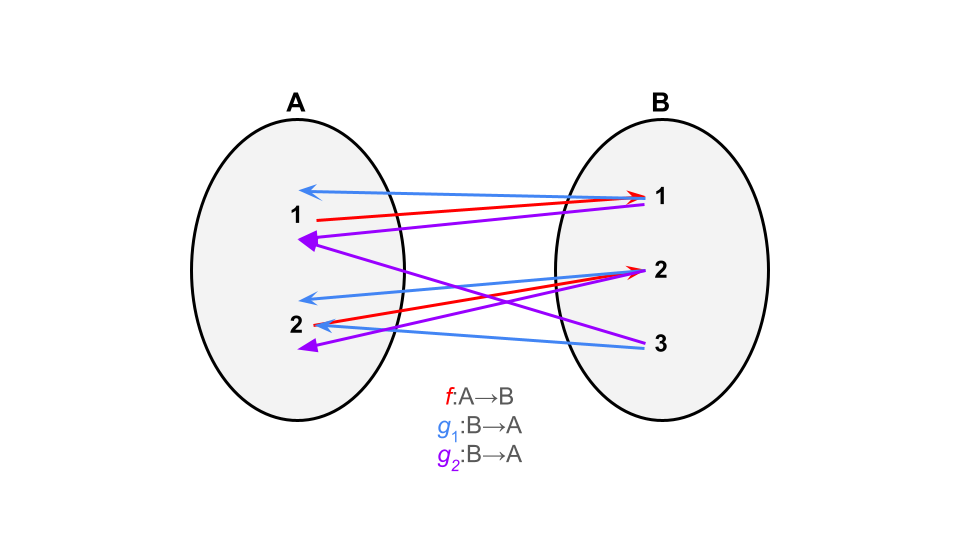
\includegraphics[scale=0.25]{M1.2.5d.png}\\
                        $g_{1}$ and $g_{2}$ are both left inverses of $f$.\\

                        A function can have more than one right inverse. $f(x) = x^{2}$ has both $h_{1}(x) = \sqrt{x}$ and $h_{2}(x) = -\sqrt{x}$ as right inverses.
                  \item Show that if $f$ has both a left inverse $g$ and a right inverse $h$, then $f$ is bijective and $g = h = f^{-1}$.\\
                        Because $f$ has a left inverse, $f$ must be injective, and because $f$ has a right inverse $f$ must be surjective (proven in part (a)), meaning $f$ is bijective.\\
                        Because $f$ is bijective, it must have an inverse $f^{-1}:B \to A$ such that $f^{-1}(b) = a$, where $f(a) = b$.\\
                        By substituting, we get that $f^{-1}(f(a)) = a$ for all $a \in A$. This means $f^{-1}$ is a left inverse of $f$, and because a function can have only one left inverse, $f^{-1} = g$.\\
                        We can also substitute to reach $f(f^{-1}(b)) = b$, meaning $f^{-1}$ is a right inverse of $f$. $h:B \to A$ is also a right inverse of $f$, so $f(h(b)) = b$. $f$ is injective, so $h(b) = f^{-1}(b)$ for all $b \in B$, so $h = f^{-1}$.
                        $g = f^{-1}$ and $h = f^{-1}$, so $g = h = f^{-1}$.
            \end{enumerate}
      \item Let $f: \mathbb{R} \to \mathbb{R}$ be the function $f(x) = x^{3} - x$. By restricting the domain and range of $f$ appropriately, obtain from $f$ a bijective function $g$. Draw the graphs of $g$ and $g^{-1}$.\\
            Let $g:[1, \infty) \to [0, \infty)$ be the function $g(x) = x^{3} - x$.\\
            \begin{tabular}{c c}
                  $g(x)$                                & $g^{-1}(x)$                                  \\
                  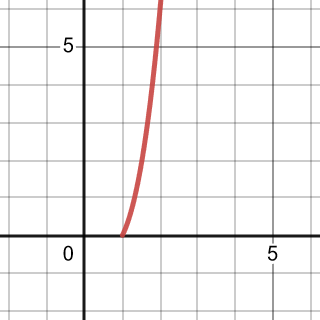
\includegraphics[scale=0.25]{M1.2.6g} & 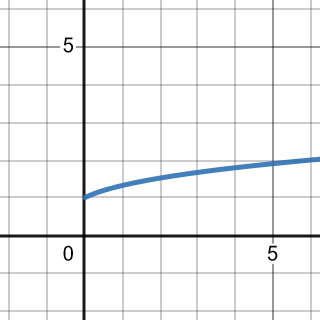
\includegraphics[scale=0.25]{M1.2.6ginv.png}
            \end{tabular}

\end{enumerate}


\end{document}